\documentclass{article}
\usepackage[english]{babel}
\usepackage[english]{isodate}
\usepackage[style=ieee,backend=bibtex]{biblatex}
\addbibresource{9_references-scholar.bib}
\addbibresource{9_references-other.bib}

\usepackage[margin=1in]{geometry}
\usepackage{hyperref}
\usepackage{booktabs}
\usepackage{multirow}
\usepackage{tikz}
\usepackage{pgfplots}
\usepackage{standalone}
\usepackage{xcolor}
\usepackage{standalone}
\usepackage{tabularx}
\usepackage{subfig}
\usepackage{csquotes}
\usepackage{float}

\definecolor{darkblue}{rgb}{0, 0, 0.5}
\hypersetup{colorlinks=true,citecolor=darkblue, linkcolor=darkblue, urlcolor=darkblue}

\usepackage{charter}
\usepackage[parfill]{parskip}

\usepackage{enumitem}
\setlist[itemize,enumerate]{noitemsep, topsep=0.5pt}

% \bibliographystyle{IEEEtranN}

\newcommand{\authorref}[1]{\citeauthor*{#1} \cite{#1}}

\setcounter{tocdepth}{2}

\begin{document}

\pagenumbering{arabic}

\title{
    Multimodal Machine Learning for Road Defects Classification \\
    \small Version 0.1
}
\author{Joël Luijmes}

% \date{2021-04-08}
\maketitle

\tableofcontents

\clearpage
\section{Introduction}

In the Netherlands, public infrastructure maintainers (the state, provinces, municipalities and water authorities) have the legal responsibility for maintaining their assets. Maintaining the road means "to ensure that all roads within the area are in good condition" \cite{Wegenwet} . In this sense road maintainers are obliged to maintain facilities regularly and sustainable \cite{BurgerlijkWetbook6:174}. In order to give some guidance on how to assess the state of roads, standards are made by the national knowledge platform CROW. Among it activities the CROW prescribes road maintainers how to perform and assess road inspections \cite{CROW_147}. CROW helps maintainers in quality-driven management. 

Road maintenance is a big expenditure of the state's budget, it is annually around 2.5 - 3.5 billion (x1.000.000.000) EUR \cite{Rijksbegroting:Infrastructuur}. Depending on the type of the road, a different public body is responsible for maintaining that road. For instance, highways (indicated with A) are maintained by the state (Rijkswaterstaat), provincial (indicated with N) roads by the provinces, and local roads (indicated with street names) by municipalities. Public bodies are legally obliged to report "maintenance capital goods" in their annual budgets \cite{Wet_Besluit_Begroting}. Within the report they have to state the policy framework for maintenance and the financial implications. From this, it flows that road maintenance is planned through a multi-year plan. Programming for multi-year road maintenance requires clear insights in current road conditions. Road maintenance is a significant expensive, and being public money, it is important that it is well spent. 

\begin{figure}[ht]
    \begin{center}
    \includegraphics[height=6cm]{images/1_introduction/budget.png}
    \end{center}
    \caption{Budget for maintenance of public roads \cite{Rijksbegroting:Infrastructuur}. Budget is in billion (x1.000.000.000) EUR.}
    \label{fig:prm}
\end{figure}

Road maintenance is performed according to an annual cyclical process. The road owner or maintainer (i.e. state, province or municipality) initiates a tender for inspection. After which, an inspection company inspects the road with specialized vehicles. This vehicle contains of multiple cameras to record the road surface, infrared sensor to measure the evenness, and other types of sensors. The recorded video data is manually inspected by engineers according the prescribed CROW method \cite{CROW_147}. The inspection company delivers a report with recommendations to the road owner indicating which roads needs maintenance. On this recommendation, the road owner initiates another tender to perform the actual maintenance. Interestingly to note is that companies that can perform inspections, often also can perform the construction.

The condition of the road can thus measured through various quantifiable data sources. Below is a list given of data sources which are often used within the Netherlands for road inspection:
\begin{itemize}
\item Visual inspection: video data is manually annotated to mark damages.
\item ARAN measurements: laser sensor which measures distance between the road and vehicle across the pavement. This can be used to measure the surface unevenness or rutting.
\end{itemize}
\begin{itemize}
\item Ground penetrating radar: geophysical method which uses radar pulses to get an image of the subsurface by measuring the reflected signals. This enables to assess the quality of the asphalt and deeper layers, detect sinkholes and can detect objects below the surface.
\item Falling weight deflector: similar to ground penetrating radar, but instead of using radar pulses, a weight is dropped and reflections are measured. This method is more commonly used in civil engineering. 
\item Skid resistance: describes the force when a locked tire (i.e. a wheel that is prevented from rotating) slides along the surface. Measurements are performed by measuring the friction on the locked wheel. This method is used to detect if the road is too slippery e.g. aquaplaning.
\item Static data:  besides actual measurements, there is also static data available about roads.
\begin{itemize}
\item Materials passport describing the different layers of the road. Contains information when and how the layer was constructed and which material was used.
\item Historical maintenance reports.
\item Future date of maintenance (e.g. multi-year plan). 
\item Road intensity (how many vehicles travel the road).
\end{itemize}
    
\end{itemize}
Keeping track of these various sources of data is cumbersome. From experience it appears that  many road owners try to manage this data manually, that is without any specialized software. However, there are some tools in the industry to support their workflow. These software tools are known as "asset management software" or "management systems" . One of the available tools is Predictive Road Maintenance (PRM), a platform for data driven asset management (see figure \ref{fig:prm}). This tool is developed by AssetWorx \footnote{Pronounced as Asset Works}, this is also the startup where this thesis is written. PRM is created during an incubator program known as 'Startup in Residence' funded by the province Overijssel \cite{Residense2020}. As of now (Jul. 2021), PRM is only used by the province Overijssel, but AssetWorx is in active negotiation with other provinces and municipalities for adoption. The ultimate goal is to create an uniform data platform for road maintainers. The idea is to be a disrupter of the industry by providing data driven insights in road quality, maintenance and planning as an independent organization (i.e. not one of existing engineering firms). 

\begin{figure}[ht]
    \begin{center}
    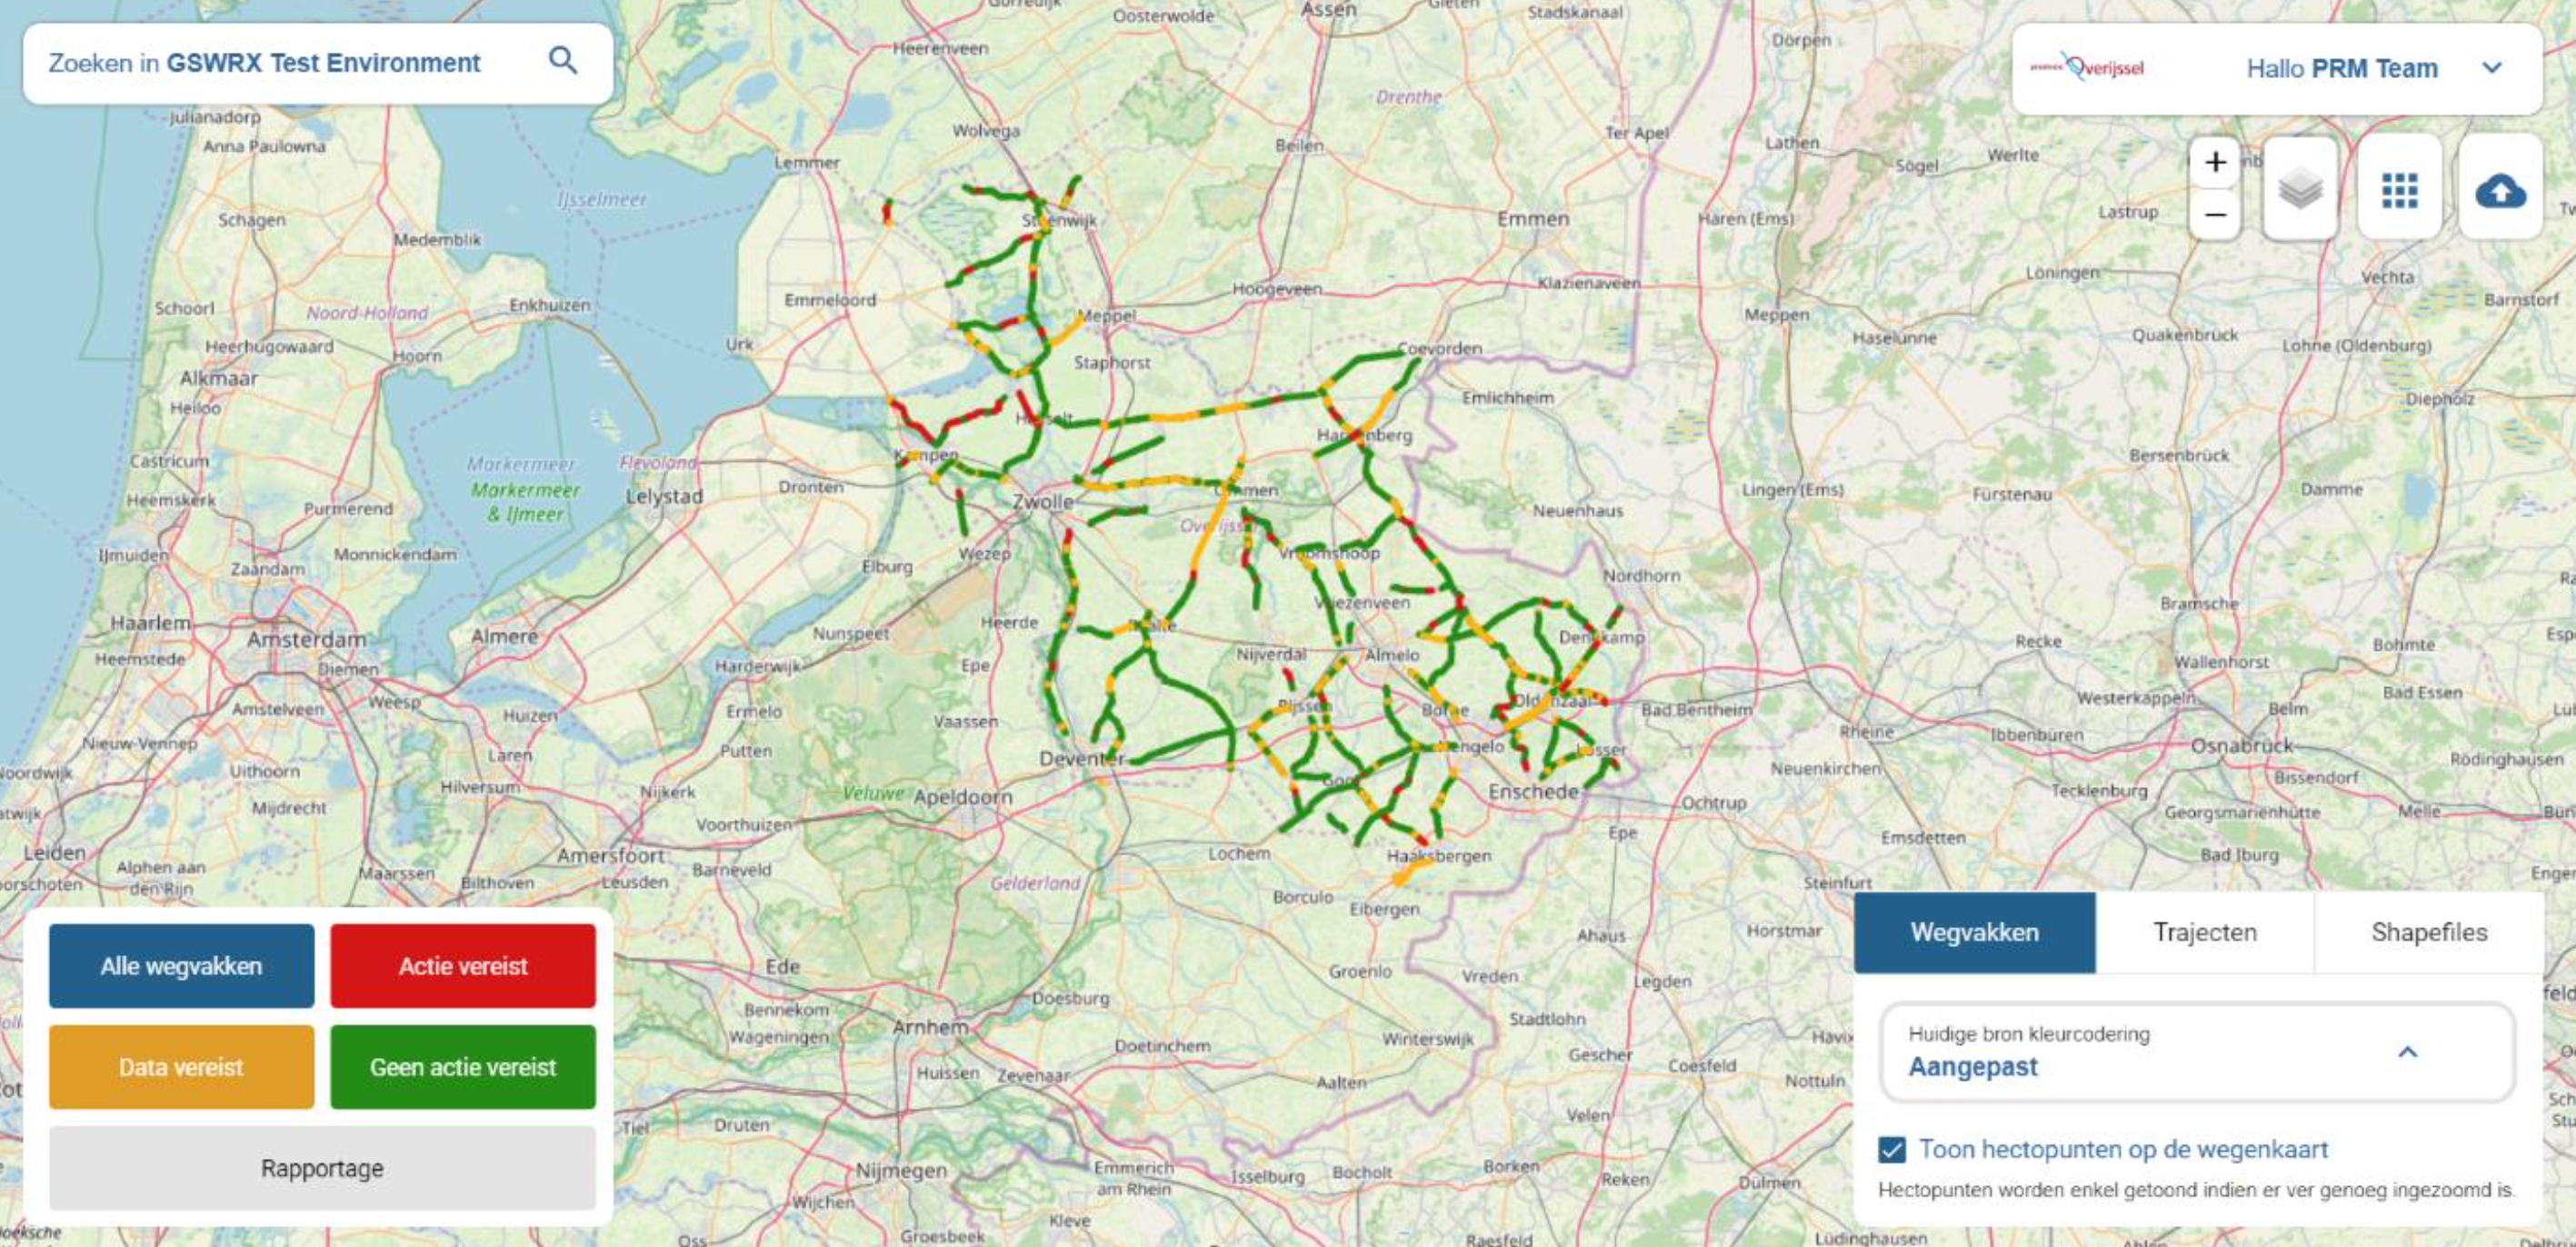
\includegraphics[height=6cm]{images/1_introduction/prm-overview.png}
    \includegraphics[height=6cm]{images/1_introduction/prm-detail.png}
    \end{center}
    \caption{Screenshots of Predictive Road Maintenance (PRM) software.}
    \label{fig:prm}
\end{figure}


\subsection{Relevance}

Although there are other asset management tools in the market, they typically only incorporate one or two data sources. PRM however is designed to operate on all kinds of data, as long the data can be geographically grounded (e.g. GPS coordinates). Currently, almost all road assessment rely on visual inspections based on the CROW systematic \cite{CROW_147}. This is an intensive procedure which largely relies on experience and intuition of the inspectors and maintainers. The cycle of tendering -> inspection -> tendering -> maintenance, typically takes one year. However, when there is a damage in the pavement, the severity of that damage may increase as it remains not repaired. For instance, a pothole starts relatively small but over time, as more traffic passes, it may become a significant damage in the road that eventually affects the drivers. Repairing a small pothole is easy and quick, but as the damages increases, so does the financial costs of repairing a road. Therefore, timely monitoring of road damages saves costs for the maintainer while increasing comfort of driving and safety.

AssetWorx aims to systematically and continuously collect data on roads instead of the conventional annual cycle of inspection and maintenance. Data is manually collected through a sensor box, more details follow in later section. The collected data is then processed to automatically determine the state of the road. In order to determine that state, research (in form of this thesis) is performed to automatically detect road surface damages. None of the existing management tools incorporate this functionality. From online articles, it seems that some construction companies try to pursue this for their own proprietary tools. Automatic detection of road surface defects thus yields a large business value for AssetWorx. When road defects can be detected in a short period, it means that repair costs are minimum, thus yielding a large societal value for road maintainers as well.

Although automatic defect detection have societal and business value, it is scientifically not something new. However, existing literature only utilizes a single source of data (unimodal) to detect damages. For this research, we are collecting various types of data: visual, sound, GPS, accelerations and the CAN bus. The CAN bus is the information bus used connecting different components within a car. Multimodal fusion aims to integrate data of different sources and types in a unified representation \cite{Baltrusaitis2017}. The idea is that by fusion richer information is provided than a single modality can provide. In order to scope the research, we will only be looking at fusing visual and accelerometer data. Within existing literature on road defects detection, multimodal fusion has not been applied. Additionally, fusion of accelerometer and visual data has only been researched in the context of odometry / robot navigation, not to detect damages or objects for that matter. Finally, fusion of visual and accelerometer data is an interesting challenge due time synchronization issue. As the image at timestamp $t_{visual}$ looks ahead, while the accelerometer measures the accelerations at some delay $t_{acc} = t_{visual} + \tau$. 


\subsection{Research Questions}


During this research we are collecting various types of data. To scope our research we only will be looking at fusing visual and accelerometer data. Reason for this is that these sources can be collected in the most reproducible way. The accelerometer is positioned at fixed point inside the vehicle, and a smartphone is attached to the windshield in a conventional holder. Although we also collect sounds and CAN-bus information, these sources are neglected for now. Road noise may not be reliable due conditions (radio, talking), and CAN-bus information differs for each vehicle.

Fusing these visual and accelerometer data is interesting. Visual data can only be recorded in good conditions (i.e. weather and lighting). Complementary, vibrations can always be measured regardless of external conditions. At the same time, interpreting vibration data might pose a difficult task for humans. Combining both data sources helps to interpret the data. With that in mind, this thesis aims to answer the following research question

\begin{itemize}
\item \textbf{RQ: How can we fuse visual and accelerometer data in an end-to-end multimodal deep learning model to classify road surface defects?}
\end{itemize}

In order to answer this question, we can divide it into smaller parts. First of all, to my knowledge, no research has been performed to use multimodal data for detecting road surface defects. However, there have been extensive research on uni-modal data (mostly based on images). To get a better understanding of this field, the first sub question is:

\begin{itemize}
\item \textit{SQ1: What kind of data and algorithms are used to detect road surface defects?}
\end{itemize}

The research is focused on fusing visual and vibration data. In order to fuse these data types, we need to make good representations on each respective data source. The visual data is most easily interpreted by humans. As road surface defects are basically objects in an image, the following research questions is formed:

\begin{itemize}
\item \textit{SQ2: What is state of the art in visual object detection?}
\end{itemize}

Although data fusion hasn't been used in detecting road surface defects, multimodal fusion has been used for visual and accelerometer data.

\begin{itemize}
\item \textit{SQ4: What is the state of the art in combining visual and sensor data for multimodal data fusion?}
\end{itemize}

Specifically we are interested in time synchronization to combine visual and vibration data. Since the camera records front-faced at timestamp $t_{visual}$, the vibration data at $t_{acc}$ is measured with some delay $\tau$. 

\begin{itemize}
\item \textit{SQ5: How to calculate the delay between front-faced visual data and the accelerations of the traveling vehicle?}
\end{itemize}


\subsection{Contributions}

TODO: Write out in actual words / alineas

Contributions of this thesis are as follows:
\begin{itemize}
\item Entrepreneur / social; 
\begin{itemize}
\item Automatic detection of road damages -> saves costs
\item Example data architecture of processing vehicle data on large scale
\end{itemize}
\item Scientific:
\begin{itemize}
\item Novel end-to-end model to detect road surface defects
\item Novel method to fuse future detected object with accelerometer data
\item Open-source code / data?
\end{itemize}
\end{itemize}



\subsection{Remainder}

The remainder of this thesis is structured as follows:

\begin{enumerate}
\addtocounter{enumi}{1}
\item \textbf{Literature} presents the current literature known on the subject. It answers the theoretical research subquestions 1-3. 
\item \textbf{Methodology} explains the methodology that is used during this thesis.
\item \textbf{Data Processing} presents the various data engineering activities required to record and process the data in order to make predictions.
\item \textbf{Multimodal Fusion} deals with the performed experiments.
\item \textbf{Discussion} interprets the results.
\item \textbf{Conclusion} concludes the thesis, and provides some suggestions for future activities.

\end{enumerate}


\clearpage
\section{Literature}

\subsection{Multimodal Machine Learning}

We experience the world as multimodal: we see objects, feel vibrations and hear sounds. Modality refers to the way in which something happens or is experienced. A research problem is characterized as multimodal when it includes multiple of such modalities \cite{Baltrusaitis2017}. Commonly referred example of an interesting multimodal experience is the McGurk effect \cite{McGurk1976}. This is the perception between hearing and vision in speech. When we hear the syllable /ba/ while watching the lips of someone saying /ga/, we perceive it as /da/. 

Multimodal research has a long history from audio-visual speech recognition to more recent interest due deep learning \cite{Ngiam2011}. It has been proven that multimodal learning algorithms performs really well on various tasks, such as (audio-visual) speech recognition \cite{Noda2014}, image sentence matching \cite{Ma2015} and RGB-D object recognition \cite{Eitel2015,Xu2017,Sindagi2019}.

\authorref{Baltrusaitis2017} identified five challenges dealing with multimodal machine learning:
\begin{enumerate}
\item \textbf{Representation}: how to represent and summarize multimodal data to exploit the complementary and redundancy of multiple modalities. Distinction is made between \textit{joint representation} - which combines unimodal signals in the same space, and \textit{coordinated representation} - which processes unimodal signals separately, but enforces similarity constraints. See figure \ref{fig:structure-joint-coordinated} below for an illustration.
\item \textbf{Translation}: how to translate data from one modality to another. For example, given an image the task is to give a caption to describe the image.
\item \textbf{Alignment}: how to identify direct relations between (sub)elements from multiple modalities. For example, given an image and a caption, find the area in the image describing the caption.
\item \textbf{Fusion}: how and when to fuse / join information from multiple modalities. Historically the original topics of multimodal machine learning, with emphasize given on early-, hybrid- and late-fusion.
\item \textbf{Co-learning}: how to transfer knowledge between modalities. For example by exploiting knowledge of a rich modality, to aid modelling of a less describing modality.
\end{enumerate}

\begin{figure}[ht]
\begin{center}
\includegraphics[width=\textwidth,keepaspectratio]{images/2_literature/joint-vs-coordinated-representations.png}
\end{center}
\caption{Structure of joint and coordinated representation \cite{Baltrusaitis2017}}
\label{fig:structure-joint-coordinated}
\end{figure}

For my thesis I think the most important challenges will be relating to representation, alignment and fusion.

To my knowledge there hasn't been any research performed on multimodal fusion on road defects. In the broader sense, multimodal fusion has been applied to detect damages. Examples of which are: combining audio-visual data to detect conveyor belt damages \cite{Che2021}, gearbox fault detection based on vibrations and acoustic signals \cite{Li2016}. See \cite{Olivan2018} for more examples of data fusion in industry.

Further exploratory research shows that visual and accelerometer (IMU) data are mainly fused in odometry. Odometry is the use of motion sensors to estimate the location over time, often used in intelligent robots. The purpose of fusing these data types is often used for dead-reckoning. Which is the process of calculating the current position based on previously known position, e.g. can be used when GPS connection is unstable / lost \cite{Jiang2017,Brossard2020}.

Although mutimodal fusion hasn't been applied to road surface defects, something related has been done by \authorref{Lekshmipathy2020}. In the paper the researchers compared the results of classifying defects based on vibrations (accelerometer) with a vision-based method. They find that vision-based method outperforms the vibration-based method. Nevertheless, they argue that vibration-based method is still useful. Vision based approach only works during daytime (under correct lighting), whereas vibrations can always be collected regardless of lighting situation or weather.

\subsubsection{Conclusion}
Although multimodal machine learning is not something new, it hasn't been applied in the domain of road maintenance. To my knowledge the fusion of accelerometer and visual data hasn't been used yet for detecting damages in general. The closest comes the work of \authorref{Lekshmipathy2020}, where they compare vibration- and visual-method for classifying road defects. My thesis aims to fill the gap by applying multimodal machine learning to detect road damages. 

% ********************************************************************************
% ********************************************************************************
% ********************************************************************************

\subsection{Automatic Road Defects Classification}

Preliminary literature review shows that there is a whole field about data driven road quality assessment. This field is driven by the fact that traditional methods of assessing road quality is costly, due requirement of specialized equipment. Researchers focuses on alternative forms to collect the data by cheaper methods, such as smartphones and sensor boxes. In current literature we identified the following \textit{subfields} based on the type of data that is used:

\begin{enumerate}
\item Road surface defects: based on image data (e.g. cracks).
\item Roughness evaluation: based on accelerometer / gyroscope (e.g. IRI).
\item Noise labelling: based on microphones.
\end{enumerate}

\begin{figure}[h!]
\begin{center}
\includegraphics[height=5cm,keepaspectratio]{images/2_literature/aran.png}
\end{center}
\caption{Automatic Road Analyzer (ARAN) is specialized vehicle to gather data about the road surface \cite{Gupta2020}.}
\end{figure}

\subsubsection{Road surface defects}
Road surface defects or crack detection is a field trying to automatically classify damages based on image data. Usually the source of these images are smartphones. Additionally, there is also research performed using blackboxes (dashcams) and Kinect, where the latter is also able to measure depth. Research evolved from pictures taken from a top-down view, to front-faced view to support gathering data while driving.

In \authorref{Jahanshahi2012} the authors uses a Kinect sensor to collect image and depth data. Recording of the road has been performed from a top-faced view. The authors classify cracks, potholes and patches with accuracy scores of respective 78\%, 92\% and 90\%. By including depth measure, the problem is relatively trivial as classification is done by checking if the depth is greater than some threshold. 

\authorref{Zhang2016} proposes the first model (to their knowledge) which uses deep learning to detect road cracks. Their data has been collected by smartphones, although not mentioned explicitly, it seems their data has been collected from top-faced view and from deliberate pictures of a known defect. Related is \authorref{Zhang2017} where the authors use 3D pavement images and deep-learning network to classify road cracks. Their research is focused on acquiring pixel-level accuracy, with the aim that the model is able to tell the size and dimensions of the crack.

\authorref{Chatterjee2018} perform road crack detection on cycle roads in Germany. Their data has been collected from a front-faced view. Extensive feature extraction is performed with various computer vision based algorithms before making classifications with machine learning models. 

\authorref{Maeda2018} researched the possibilities of road damage classification by using smartphone images. Data was collected conventional smartphone holder for cars with a front-faced view while driving. They extensively collect data about Japanese roads and publishes their data and their trained model. This is also the first paper which makes distinctions between more types of road damages, such as fading line markings and distinction between lateral / longitudal cracks. The research is continued in \authorref{Arya2020-transfer}, where additional data is collected in Czech Republic and India. With the aim to see if their model is able to transfer learn on this new data. In order to further improve the published model, \authorref{Maeda2020} uses a generative adversial network to augment more data and retrain the model. Finally, a competition is held with their collected data \cite{Arya2020-competition}. The goal is to push the state of art of road damage detection forward. The competition consisted of two challenges: 1) classification (what kind of damage) and 2) detection (where is the damage). This competition yielded a model with an average F1 score of 0.67 for all classes. Greatly improving the original model, which yielded at best a F1 of 0.40 for only a single type of damage.

Besides making classifications, there has also been research focusing on segmenting the damages into crack and non-crack parts. \authorref{Dung2018} uses a fully convolutional neural network and \authorref{Bang2019} uses a encoder-decoder network.


\subsubsection{Roughness evaluation}
A different research field is centered around measuring the road roughness. Which is defined as the deviation of the surface from the true planar surface. This deviation affects vehicle dynamics and ride quality. Two methods to classify the roughness of a profile are the International Roughness Index (IRI) \cite{Sayers1986} and the International Standards Organisation (ISO) \cite{ISO8608} classification. There are various methods for measuring the profile data, typically used by road maintenance are inertial profilers. This is a device which scans the surface of the pavement with lasers to measure the distance, example of this is the Automatic Road Analyzers (ARAN) vehicle.

Research is focused on replacing these expensive devices with accelerometers, often those found in smartphones \cite{Hanson2014,Buttlar2014,Gupta2020}. Measuring the profile is done by filtering out the vertical accelerations and calculate the roughness accordingly to the IRI or ISO specification. Additionally, using the accelerometer it is also possible to identify potholes, bumps and patches \cite{Lekshmipathy2020}. 

Limitation of this method is that the accelerometers need to be calibrated, which is also deeper described in \cite{Gupta2020}. \authorref{Jeong2020} therefore argue that requirement of calibration hinders the widespread use of the technology. They propose a novel method using a convolutional neural network to eliminate the requirement of calibration.


\subsubsection{Noise labelling}
Quality of the road surface influences noise and vibrations emissions caused by the interaction between the tires and the road. In the EU, member states are required to publish noise maps for roads every five years \cite{EU2002}. Monitoring can be done with a vehicle equipped with a Close Proximity (CPX) trailer. This devices measures the emitted sounds from a reference tire.

\begin{figure}[ht]
\begin{center}
\includegraphics[height=5cm,keepaspectratio]{images/2_literature/cpx-trailer.jpg}
\end{center}
\caption{Close Proximity (CPX) trailer measures the sounds emitted by reference tyre \cite{MP2020}.}
\end{figure}

\authorref{Hauwermeiren2019} try to replicate the results of CPX measurements by using a sensor box containing a microphone. This microphone is located inside the trunk of the car. The authors were able to accurately estimate the road texture. However the with main limitation is that the data was collected under good conditions, such as no background radio or talking. This research is later continued, where the authors use multiple vehicles and more realistic driving conditions. They found that below 1600 Hz, their results differ from CPX less than the difference between bi-annually repeated measurements, indicating it is possible to perform this measurement using microphones \cite{Hauwermeiren2021}.


\subsubsection{Conclusion}
Automatic classification of road defects have been extensively researched. Main topic of interest is the usage of low-cost devices such as smartphones to collect the data. From the literature we find that only the following types of defects are classified: cracks, patches, holes and faded line markings. Raveling, rutting and skewed signs haven't been researched yet to my knowledge. From the field of classifying road defects we can draw a lot of knowledge to use for my thesis. Especially this is useful when to model the right representations of the data to use for multimodal machine learning.

% ********************************************************************************
% ********************************************************************************
% ********************************************************************************

\subsection{Object Detection}

% ********************************************************************************
% ********************************************************************************
% ********************************************************************************

\subsection{Accelerometer Signal Processing}

% ********************************************************************************
% ********************************************************************************
% ********************************************************************************

\subsection{Alignment of Sources in Multimodal Fusion}
\clearpage
\section{Research Methodology}

The final solution for the company is a model to assess road quality based on different sources of data. Methodologically we can see this as a design problem. In which the research goal is to design, develop and evaluate an artefact (solution)\cite{Hevner2004}. In order to ensure a certain degree of scientific rigor, a design science methodology is used \cite{Versloot2019}.

In this respect Hevner et al. \cite{Hevner2004} is commonly referred to, in which researches perform cyclical process of development and evaluation. However, Sein et al. \cite{Sein2011} state that traditional design research has drawbacks in which scientific rigor is more valued than organizational value. Thereby failing to recognize that the artefact actually emerges from interaction with the organization. In their paper, the authors propose a new method called Action Design Research (ADR). This method based on a more iterative approach. This approach reflects the premise that IT artefacts are shaped by the organization, both during development and use. It conceptualizes research process as the interwoven activities of: building the IT artefact, intervening in the organization and evaluating it concurrently \cite{Sein2011}.

ADR consists of the following four stages \cite{Sein2011}.
\begin{enumerate}
\item \textbf{Problem Formulation}: identifies and conceptualizes a research opportunity. The trigger is a problem perceived or anticipated by the researchers. Input can come from practitioners, end-users, researchers, existing technology and/or review of prior research.
\item \textbf{Building, Intervention, and Evaluation}: iterative process which interweaves building the IT artefact, intervention in the organization, and evaluation (BIE). The problem framing of stage one is used to generate an initial design of the IT artefact which is further shaped by organizational use and subsequent design cycles. During BIE, the problem and artefact are continually evaluated.
\item \textbf{Reflection and Learning}: recognizes that the research problem involves more than simply solving a problem. Conscious reflection on the problem framing, theories chosen, and the emerging ensemble is critical to ensure contributions to knowledge are identified. This is a continuous stage which run in parallel with the first two stages.
\item \textbf{Formalization of Learning}: has the goal to generalize the learning. Making the learning from specific-and-unique to a generic-and-abstract. 
\end{enumerate}

This thesis proposal states the problem formulation that road quality assessment is a costly and labor-intensive procedure (see section \ref{section:problem}). On approval of this proposal we'll move to the following stages. \textit{Building, Intervention, and Evaluation} is the experimental process in which the activities from above are performed. This stage will be done in accordance with the organization. With the purpose to make artefacts in such way that they are usable by the organization. The following stage \textit{Reflection and Learning} is done in accordance with the university of which the contributions and learnings are written down in my thesis. Finally the stage \textit{Formalization of Learning} will be done in the discussion and reflection of my thesis.

\clearpage
\section{Data Collection and Processing}

Data collection for this research was initially done using a sensor box connected with a webcam. Specifically, an AutoPi \cite{AutoPi} was connected with the OBD-2 port of the vehicle. Through this port, the AutoPi is able to all kinds of vehicle data such as RPM, speed, engine temperature etc. It depends on the specific vehicle which data sources are available. Additionally, the AutoPi is equipped with an accelerometer and GPS sensor. The OBD-2 connector is mandatory in all cars since 2004 in the EU\cite{EU1998} , and therefore it seemed like a reliable approach to collect data. With this method, XXX trips were collected. Unfortunately, there were two problems with this collection setup. First, the used webcam was unable to accurately record visual data due variable lighting changes. Initially, this was solved by recording visual data with an external smartphone. However, the second issue was more problematic. For this research we want to fuse visual and accelerometer data. However, the accelerometer data from the AutoPi was only sampled at a relative low frequency of 12.5 Hz. Further data processing operations would be problematic at such low sampling frequency.

Since the visual data was already collected with a smartphone. It was decided to also collect accelerometer and GPS data with that same smartphone. Specifically that smartphone is an Apple iPhone 12 Mini. The phone is located in a generic used phone holder attached to the windshield, see figure \ref{fig:smartphone-collector}. To  collect the data an open-source app was modified and deployed on the smartphone.\footnote{See \cite{ios_logger} for modified fork and \cite{ios_logger_original} for original. Main modification is to keep the smartphone from sleeping while collecting data.} With this app, the following data is collected:
\begin{itemize}
\item Visual data: recorded in 1280 x 720 at 30 frames per second. Each frame contain a specific timestamp when that frame was collected.
\item Accelerometer data: sampled at 100 Hz. 
\item Location data: sampled at 1 Hz. Contains GPS coordinates, but also travel heading and traveling speed.
\end{itemize}


\begin{figure}[H]
\begin{center}
\includegraphics[width=\textwidth,keepaspectratio]{images/4_data/smartphone-setup.jpg}
\end{center}
\caption{Setup of smartphone to collect data.}
\label{fig:smartphone-collector}
\end{figure}

Data collected from the first approach is kept and visual data is still used to label visual objects. The processing steps for other sensor data (GPS and accelerometer) from the AutoPi and smartphone are equal. However, when noting sensor specifics, the latter collecting approach is assumed unless otherwise stated.


\subsection{Data Platform Architecture}
Currently AssetWorx lacks the infrastructure and architecture to process the collected data. In order to systematically process the collected data various data pipelines are designed. These pipelines can be holistically viewed as as a \textit{data platform architecture}. Implementation and execution of this platform is done on Google Cloud Platform (GCP) by using certain services GCP provides i.e. Kuberenetes and BigQuery. To orchestrate the various steps, Prefect\cite{Prefect} is used. Prefect is a dataflow automation tool. Although it is capable to orchestrate large scale workflows for data processing, it also provides an easy to use library to create and run workflows / pipelines locally.

The designed approach takes a modern data platform architecture with loosely coupled layers. A data architecture is either modelled based on the used data sources or on the specific areas (or maturity) of the data. In this case, the latter approach is used as later processing steps use data from multiple sources. Maturity refers to the readiness of consumption of that data. Data comes in raw form, but often needs some transformations (cleaning, deduplication) to make it ready for consumption e.g. analysis.  Below in figure \ref{fig:data-platform-architecture} an overview is given of the data platform.

\begin{figure}[H]
\begin{center}
\includegraphics[width=0.95\textwidth,keepaspectratio]{images/4_data/data-platform.png}
\end{center}
\captionsetup{width=.95\textwidth}
\caption{Overview of data platform architecture.}
\label{fig:data-platform-architecture}
\end{figure}

\begin{enumerate}
\item Ingestion Layer: getting the data into the data platform. Data is manually pulled from the smartphone to a laptop. From this laptop the data is uploaded using automated scripts. Note, to ensure privacy concerns, visual data is first anonymized to remove PII data. Although this layer is not strictly within the Google Cloud Platform, it is still part of the total data platform.
\item Storage Layer: data is stored in the data platform in two services, BigQuery - a managed data warehouse solution and Cloud Storage - a generic object store. Within these two services, the data is split in three layers denoting the maturity of the data.
\begin{enumerate}
\item Raw / landing: contains the data in the form it is collected by the smartphone.
\item Staging: intermediate layer, data is processed in more useful form but not ready for consumption.
\item Production / marts: contains data ready for consumption, e.g. analyzing data and training models.
\end{enumerate}
\item Processing Layer: consumes data from the storage layer and processes it. For instance, data transformations between different areas (raw, staging, marts) or training models. Some processing steps are fully implemented with SQL and ran in BigQuery, other rely on custom Python code and are ran in Kubernetes cluster.
\end{enumerate}

In table \ref{tab:data-pipelines} all the data pipelines are listed with a description of their operation. In figure \ref{fig:data-pipelines} the pipelines are visualized (TODO: outdated). Many data pipelines are relatively straightforward and don't need further explanation than listed in the table. However, there are a few interesting processing operations further described below. The data pipelines are grouped per used data source. First we cover GPS data, then the accelerometer and finally the visual data.

% Please add the following required packages to your document preamble:
% \usepackage{booktabs}
% \usepackage{graphicx}
\begin{table}[h!]
\resizebox{\textwidth}{!}{%
\begin{tabular}{@{}p{0.25\linewidth}llp{0.6\linewidth}@{}}
\toprule
Name &
  Source &
  Destination &
  Description \\ \midrule \midrule
Ingest Accelerometer &
  \begin{tabular}[c]{@{}l@{}}Landing\\ Cloud Storage (jsonlines)\end{tabular} &
  \begin{tabular}[c]{@{}l@{}}Landing\\ BigQuery\\ \textit{raw\_accelerometer}\end{tabular} &
  Loads raw records from Cloud Storage into BigQuery table. \\ \midrule
Ingest GPS &
  \begin{tabular}[c]{@{}l@{}}Landing\\ Cloud Storage (jsonlines)\end{tabular} &
  \begin{tabular}[c]{@{}l@{}}Landing\\ BigQuery\\ \textit{raw\_gps}\end{tabular} &
  Loads raw records from Cloud Storage into BigQuery table. \\ \midrule
Ingest Wegdeel &
  \begin{tabular}[c]{@{}l@{}}External\\ Postgis\end{tabular} &
  \begin{tabular}[c]{@{}l@{}}Landing\\ BigQuery\\ \textit{raw\_wegdeel}\end{tabular} &
  Loads road sections (wegdeel) from Postgis database into BigQuery table. \\ \midrule
Ingest Frames Labels &
  \begin{tabular}[c]{@{}l@{}}Landing\\ Cloud Storage (txt)\end{tabular} &
  \begin{tabular}[c]{@{}l@{}}Landing\\ BigQuery\\ \textit{raw\_frames\_labels}\end{tabular} &
  Loads manually label annotations into BigQuery table. \\ \midrule
Ingest Label Lookup &
  \begin{tabular}[c]{@{}l@{}}Landing\\ Cloud Storage (txt)\end{tabular} &
  \begin{tabular}[c]{@{}l@{}}Landing\\ BigQuery\\ \textit{raw\_label\_lookup}\end{tabular} &
  Loads manually label definitions into BigQuery table. \\ \midrule \midrule
Determine Trips &
  \begin{tabular}[c]{@{}l@{}}Landing\\ BigQuery\\ \textit{raw\_gps}\end{tabular} &
  \begin{tabular}[c]{@{}l@{}}Staging\\ BigQuery\\ \textit{stg\_gps}, \textit{stg\_trips}\end{tabular} &
  Parses from GPS records distinct trips the car has travelled (further described below). \\ \midrule
Snap Trips to Roads &
  \begin{tabular}[c]{@{}l@{}}Staging\\ BigQuery\\ \textit{stg\_trips}\\ \\ External\\ Bing\end{tabular} &
  \begin{tabular}[c]{@{}l@{}}Staging\\ BigQuery\\ \textit{stg\_trips\_snapped}\end{tabular} &
  Snap the preprocessed GPS records to actual roads (further described below). \\ \midrule
Filter Road Sections &
  \begin{tabular}[c]{@{}l@{}}Landing\\ BigQuery\\ \textit{raw\_wegdeel}\end{tabular} &
  \begin{tabular}[c]{@{}l@{}}Staging\\ BigQuery\\ \textit{stg\_road\_section}\end{tabular} &
  Filter the road sections that are actually in use. \\ \midrule
Create Label Lookup &
  \begin{tabular}[c]{@{}l@{}}Landing\\ BigQuery\\ \textit{raw\_label\_lookup}\end{tabular} &
  \begin{tabular}[c]{@{}l@{}}Staging\\ BigQuery\\ \textit{stg\_label\_lookup}\end{tabular} &
  Converts ingested definitions to lookup table in order to join with annotated frames.\\ \midrule
Video to Frames &
  \begin{tabular}[c]{@{}l@{}}Landing\\ Cloud Storage (mov)\end{tabular} &
  \begin{tabular}[c]{@{}l@{}}Staging\\ Cloud Storage (jpg)\end{tabular} &
  Extracts separate frames from the recorded video (1 frame per second).\\ \midrule
Video to Frames Bootstrap &
  &
  &
  Spawns off separate jobs to process all video files in parallel.\\ \midrule \midrule
Link Trip Coordinates with Road Sections &
  \begin{tabular}[c]{@{}l@{}}Staging\\ BigQuery\\ \textit{stg\_trips\_snapped}\\ \\ Staging\\ BigQuery\\ \textit{stg\_road\_section}\end{tabular} &
  \begin{tabular}[c]{@{}l@{}}Production\\ BigQuery\\ \textit{mrt\_trips}\end{tabular} &
  Joins the snapped trips with the cleaned road sections from the BGT. \\ \midrule
Calculate Road Section Windows &
  \begin{tabular}[c]{@{}l@{}}Production\\ BigQuery\\ \textit{mrt\_trips}\end{tabular} &
  \begin{tabular}[c]{@{}l@{}}Production\\ BigQuery\\ \textit{mrt\_road\_section\_windows}\end{tabular} &
  Calculates timestamps (windows) when each road section was entered/exited per trip. \\ \midrule
Load Frames Labels &
  \begin{tabular}[c]{@{}l@{}}Landing\\ BigQuery\\ \textit{raw\_frames\_labels}\\ \\ Staging\\ BigQuery\\ \textit{stg\_label\_lookup}\end{tabular} &
  \begin{tabular}[c]{@{}l@{}}Production\\ BigQuery\\ \textit{mrt\_frames\_labels}\end{tabular} &
  Joins annotated frames with lookup table. \\ \midrule 
Load Frames Metadata &
  \begin{tabular}[c]{@{}l@{}}Production\\ Storage\end{tabular} &
  \begin{tabular}[c]{@{}l@{}}Production\\ BigQuery\\ \textit{mrt\_frames\_metadata}\end{tabular} &
  Creates a metadata table on the extracted frames (e.g. source video, timestamp and size). \\ \midrule 
Ingest Experiment Labels &
  \begin{tabular}[c]{@{}l@{}}External\end{tabular} &
  \begin{tabular}[c]{@{}l@{}}Production\\ BigQuery\\ \textit{mrt\_experiment\_labels}\end{tabular} &
  Ingests separate labels annotated by experiment runs into BigQuery. \\ \midrule 
Anonymize &
  \begin{tabular}[c]{@{}l@{}}Staging\\ Cloud Storage (jpg)\end{tabular} &
  \begin{tabular}[c]{@{}l@{}}Production\\ Cloud Storage (jpg)\end{tabular} &
  Automatically detect PII data and blur the detected objects.\\ \midrule
Anonymize Bootstrap &
  &
  &
  Spawns off separate jobs to process all source files in parallel.\\ \bottomrule
\end{tabular}%
}
\caption{Overview of all the different data pipelines.}
\label{tab:data-pipelines}
\end{table}

\begin{figure}[h!]
\begin{center}
\makebox[\textwidth][c]{\includegraphics[width=1.2\textwidth,keepaspectratio]{images/4_data/data-pipelines.png}}
\end{center}
\caption{Visual overview of the various Data Pipelines.}
\label{fig:data-pipelines}
\end{figure}


\subsection{GPS Data}
GPS data describes the location of the vehicle in coordinates. Specifically the coordinates are recorded in latitude and longitude information as notated in WGS84 standard. The data is sampled at 1 Hz. GPS data is further processed to find distinctive trips and to calculate speed and heading information of  the travelling vehicle.


\subsubsection{Determine Trips}
The GPS sensor records the location of the vehicle. After ingestion, this data is stored in raw form on Google Cloud Storage (GCS). The format of the data is stored as json lines. This is a file format where each line in the file is a single json document. Within this document the location of the vehicle is recorded with the respective time. After the data is ingested in BigQuery, the GPS data is deduplicated and distinctive trips are detected with the following algorithm. Each trip as an unique identifier, with these distinctive trips it is easier to fuse different sources i.e. querying the accelerometer data from a specific trip.

\begin{enumerate}
\item Deduplication: the GPS sensor always records location data. If the car is standing still (e.g. traffic light), the data is still recorded, resulting in duplicate records. The first step is to deduplicate the data. This is done by selecting the first record for each unique location in subsequent time series. 
\item Delta calculation: between each subsequent record the difference between time and distance is calculated.
\item Split trips: trips are detected from the consecutively records by finding records where the vehicle is stationary longer than 120 seconds. This commonly known as dwell time, and 120 seconds is often used in literature \cite{Wolf2001}.
\item Reset trips: for each first record of a trip, the delta time and distance is reset to zero.
\item Cleanup trips: to cleanup invalid data, only trips are selected with more than 5 records of data and with at least 500 meters travelled in total.
\end{enumerate}


\begin{figure}[H]
  \centering
  \includegraphics[width=0.95\linewidth]{images/4_data/trip-detection.png}
  \captionsetup{width=.95\textwidth}
  \caption{Example of trip deduction algorithm. Left shows original data, center shows after deduplicating based on the location, right shows the resulting trips.}
  \label{fig:test2}
\end{figure}




\subsubsection{Snap Trips to Roads}
GPS data is generally regarded as noisy. The accuracy of the sensor varies over time. Resulting that some coordinates are aligned on roads, while other samples are outside the road. See also figure \ref{fig:snap-trips}. This becomes an issue when we further process the data. In our case, we want to join GPS data with ground truth data for the roads. This allows to compare data from distinctive trips on the same roads, or to find build information of the roads (further described below). To cleanup this data, GPS coordinates are snapped to actual roads. The anchoring of the GPS coordinates is done with an external service. In this specific case "Snap Points to Roads" from Bing Maps \cite{Snap-Points-to-Roads} is used, but there are other APIs that perform this service.


\begin{figure}[H]
\begin{center}
\includegraphics[width=.95\textwidth,keepaspectratio]{images/4_data/snap-trips.png}
\end{center}
\captionsetup{width=.95\textwidth}
\caption{Display of snapping coordinates to roads. The blue dots are the measured GPS coordinates, and the red dots are the inferred coordinates by external service. Note that some of the blue dots are on the wrong lane or beside any roads.}
\label{fig:snap-trips}
\end{figure}

\subsubsection{Link Trip Coordinates with Road Sections}
\textit{Basisregistratie Grootschalige Topografie} (BGT) is registry in the Netherlands of "large-scale objects in the public space". This registry marks all locations and their bounding area (in coordinates) of large-scale objects such as roads, buildings and territory. The BGT is regulated by law, and is mandatory for governments to use and maintain while operating in the public space \cite{BGT}. The BGT also includes roads as \textit{road sections}. The size of a section varies to a single street bump in a town, to several hundred meters of highway. Road sections are annotated with various types of attributes, of which one is promising for this thesis. That is the material of the road: concrete, asphalt or brick. The road snapped GPS coordinates are joined to the respective road sections from the BGT.


\subsubsection{Calculate Road Section Windows}
Road sections cover a geographical area, and therefore are likely to contain multiple GPS records. Sensor data (visual and accelerometer) can only be linked with GPS through their respective timestamps. To link these data sources each road section it is calculated when that section was entered and exited. This is referred as the \textit{road section window}.

\subsection{Accelerometer Data}
Accelerometer measures acceleration, the change of velocity over time. In the smartphone the sensor measures acceleration in three axis: longitudinal (X), lateral (Y) and vertical (Z) axes. The output is in G-forces, where $1 G = 9.81m/s^2$. In stationary position, the accelerometer always measures 1G on the vertical axis due gravitational pull of the earth. Acceleration data describes the vibrations of the vehicle. However, before the data can be used, it needs to be pre-processed. Of which the most important is that the orientation of the sensor needs to be aligned with that of the vehicle. All processing steps are described down below.


\subsubsection{Re-sampling}
Re-sampling the data ensures a constant sampling frequency. This is necessary for further signal processing operations such as calculating FFT or filtering noise. This step was required when collecting data with the AutoPi (the first method). From data analysis it appeared that the AutoPi had variations in the sampling rate. With the new data collection method, the smartphone collects the accelerometer data more consistently. To ensure a consistent sampling frequency, this processing step is still applied, even for the newer collection method.

Re-sampling of the data is done by fitting a B-spline curve for all the known samples. From this spline, the data points are uniformly sampled at the expected frequency. The effect of re-sampling is shown in figure \ref{fig:accelerometer-resampling}. Note that the example in this figure was of data collected with the AutoPi. For data from the smartphone the effect is less noticable. The top blue graph shows the raw readings from the accelerometer. The bottom red graph shows the resulting data after re-sampling. Notice that the interval between readings of the top graph is variable, whereas the bottom is uniformly spaced. This approach of resampling also been used in \cite{Wu2020}.

\begin{figure}[H]
\begin{center}
\includegraphics[width=.95\textwidth,keepaspectratio]{images/4_data/accelerometer-resampling.png}
\end{center}
\captionsetup{width=.95\textwidth}
\caption{Top graph displays the raw data from the accelerometer. Bottom graph displays the accelerometer data after re-sampling. Note this example is made on data from AutoPi, where the effect is more prominent.}
\label{fig:accelerometer-resampling}
\end{figure}


\subsubsection{Realignment}
The coordinate system of the accelerometer may not coincide with that of the vehicle. Meaning, when the vehicle drives over a bump it is expected to see a acceleration in vertical axes. However, when it is not aligned, the acceleration is shown on a different axes or as a product of axes. There are two causes for this misalignment. First, we don't know how the sensor is oriented in the smartphone, making it hard to align it correctly.  As the same smartphone also needs to record the road, aligning it in such way is futile regardless. Secondly, we can't expect to place the smartphone perfectly consistent at the same angle every time in the holder. Before any of the data can be analyzed, the coordinate system of the accelerometer must be aligned with that of the vehicle. To fix this issue, a process was developed to automatically align the coordinate systems. Making it also possible to generalize collection of data to any vehicle and accelerometer sensor. This process has been inspired by \cite{accelerometer_alignment} and is also applied in \cite{Wu2020}. 

The process consists of two steps. First, the coordinate system is aligned on the vertical Z-axes using a rotation matrix $R_z$. Subsequently, the horizontal plane is aligned using a rotation matrix $R_x$. Calculating these rotation matrices is done by measuring the accelerometer sensor $a_s$when a known force is exerted on the vehicle, $a_v$. Using Euler angles we can calculate the rotation matrix to align the force $a_s$ to that of the known force $a_v$. In the figure \ref{fig:align-vectors} the two-step method is visually presented.


\begin{figure}[H]
\begin{center}
\includegraphics[width=0.95\textwidth,keepaspectratio]{images/4_data/accelerometer-alignment.png}
\end{center}
\captionsetup{width=.95\textwidth}
\caption{Figure displaying the process of aligning the axes. Zv is the Z-axes for the vehicle, Zs is the Z-axes for the sensor. Left: shows the original, unaligned situation. Middle: shows the situation after aligning the Z-axes. Right: shows situation after aligning the X-axes.}
\label{fig:align-vectors}
\end{figure}



For the first step, aligning the vertical Z-axes, the known force is the gravity of the earth. When the vehicle is stationary, the expected force is $a_v = (0, 0, 1G)$. Stationary points are found by querying the GPS data when the car is not moving. Ideally, only accelerometer data is used when the vehicle is on a level surface. As we don't have access to this information, we rely on taking the average of many samples, as it can be assumed that on average the vehicle is mostly stationary on a flat surfaces. This assumption seems plausible in the Netherlands, where the country is largely flat. See also section \ref{section:stationary-points} for detailed discussion. The rotation matrix $R_z$ is calculated to align vector $a_s$ onto vector $a_v$ as follows \cite{rotation_matrix}. 

\begin{flalign*} 
\text{Let } v &= a_s \times a_v \\
\text{Let } c &= a_s \cdot a_v \\
\text{Let } skew &=
\begin{bmatrix} 0 & -v_3 & v_2 \\ v_3 & 0 & -v_1 \\ -v_2 & v_1 & 0 \end{bmatrix} \\
R_z &= I + skew + skew^2 \frac{1}{1 + c}
\end{flalign*}

The second step is to align the coordinates system in the longitudinal X-axes. Again, we take readings of the accelerometer when a certain force is expected. In this case when the car is braking, the expected acceleration is $a_v = (-x, 0, 1G)$, where $x$ depends on the deceleration of the vehicle. Braking windows are selected based on the derived speed from the GPS coordinates. As the vertical axes is already aligned, we need to calculate a two dimensional rotation matrix $R_x$ to align vector $a'_s$ onto vector $a_v$ in the longitudinal X-axes. $a'_s$ refers to the measured acceleration after applying the rotation.

\begin{flalign*} 
\sin \theta &= a'_s \times a_v \\
\cos \theta &= a'_s \cdot a_v \\
R_x &= \begin{bmatrix} \cos \theta & -\sin \theta & 0 \\ \sin \ \theta & \cos \theta & 0 \\ 0 & 0 & 1 \end{bmatrix} \\
\end{flalign*}




\subsubsection{Noise filtering}
Accelerometer data is prone to noise. As is common with signal processing, data is first passed through a filter to obtain a clearer signal. Noise in the signal comes from vibrations generated by vehicle. Additionally, from research it is stated that specific events causes noise such as braking, acceleration and steering. Existing research uses a variety of different filter configurations to clean the data. Some apply a low-pass Butterworth filter \cite{Gupta2020}, whereas other researches use a high-pass Butterworth filter \cite{Wu2020, Janani2020}. Refer back to section \ref{sec:butterworth-filter} for detailed explication of Butterworth filter. Due the different usages, we assume that it differs per application and approach it as a possible tuning parameter.

In figure \ref{fig:filter}, various configurations of a 5th-order Butterworth filter are displayed. At the top left (blue) is the original signal while driving over a manhole. The other graphs shows the resulting signal after applying a specific configuration. For instance, the middle right (orange) is after passing the data through a high pass filter with cut-off at 2 Hz. Meaning that all frequencies below 2 Hz are filtered out. As this signal seems most clean, we use this configuration as an initial starting point. In future, other types of configurations can be applied to optimize performance. 


\begin{figure}[H]
\begin{center}
\includegraphics[width=0.95\textwidth,keepaspectratio]{images/4_data/filter-example.jpg}
\end{center}
\captionsetup{width=.95\textwidth}
\caption{Figure displaying various graphs after applying a 5th-order Butterworth filter to the accelerometer signal on the vertical Z-axis. The event shown here is when the vehicle drives over a manhole.}
\label{fig:filter}
\end{figure}




\subsection{Visual Data}
\label{sec:visual-data}

As previously mentioned the road suface is recorded with an Apple iPhone 12 Mini. The data is recorded at resolution of 1280 x 720 at 30 frames per second (FPS). The phone is located in a generic  phone holder attached to the windshield. As can be seen in the setup figure \ref{fig:smartphone-collector}, the camera angle is parallel to that of the road surface. This means that the camera also records other data than the road such as other vehicles, the sky and other surroundings. Below described are the processing steps for the visual data. Before the visual data is uploaded to the data platform it is anonymized. Therefor these processing steps are ran at local machine, as opposed to the earlier described steps.


\subsubsection{Video to Frames}
All visual data processing operations operate on single frames instead of video files. Therefore, the first step is to extract the distinctive frames from the video. The open-source tool FFmpeg \cite{ffmpeg} is used to convert the video to the frames. The frames are linked with their respective timestamps as recorded by the data collection app.


\subsubsection{Anonymization}
Although not intentional, the camera may record other cars, persons and other PII data. To safeguard any privacy concerns, the data is anonymized. This is done by blurring PII data from the individual frames. Detection of PII data happens with pre-trained object detector YOLOv5 model \cite{Jocher2021}. This model is trained on COCO dataset, and thus is capable of detecting various classes among which are: [person, bicycle, car, motorcycle, airplane, bus, train, truck, boat. After the frames are anonymized, the frames are uploaded to the data platform. 


\subsubsection{Optical Flow}
Visual and accelerometer data can be synchronized when the same events are present in both modalities. Dense optical flow estimates the acceleration between two frames. Using optical flow it is possible align visual and accelerometer data. This has also been further described in section \ref{section:synchronization}. 

For each of the extracted frames, the optical flow is calculated. This is done with the Farneback algorithm\cite{Farnebäck2003}. The average of output is taken which results in a 2D vector field, describing the full motion of the frame in horizontal X- and vertical Y-axis. In figure \label{fig:optical-flow} the results are shown. At the top the input frame is shown in raw form, and after calculating the optical flow. The bottom graphs compares the full vertical optical flow with that of measured accelerometer data. Although it is not visible in on this graph, there exists a small delay between the modalities due time synchronization. Referred to as $\tau_{capture}$. Synchronization of these modalities is tackled in section \ref{sec:capture-time-synchronization}.

\begin{figure}[H]
\centering
\subfloat{{\includegraphics[width=0.45\textwidth,keepaspectratio]{images/4_data/original.jpg} }}%
\quad
\subfloat{{\includegraphics[width=0.45\textwidth,keepaspectratio]{images/4_data/optical-flow.jpg} }}%
\label{fig:optical-flow}
\end{figure}

\begin{figure}[H]
\centering
\includegraphics[width=0.95\textwidth,keepaspectratio]{images/4_data/optical-flow-graph.jpg}
\end{figure}




 

\clearpage
\section{Multimodal Machine Learning}

The aim of this thesis is to detect road defects using multimodal machine learning. As described earlier in section \ref{section:multimodal-ml}, multimodal means that there are multiple data sources. In this case, it deals with visual- and accelerometer data. There are three points in the pipeline where the modalities can be fused: early- middle- or late fusion \cite{Baltrusaitis2017}. However, a model can also be trained on the respective modality, i.e. training a classifier solely on visual data. This makes sense as it can act as a baseline to multimodal learner. Therefore this thesis researches three tracks:
\begin{enumerate}
\item Visual only: based on the visual data an object detector is trained to classify road anomalies.
\item Accelerometer only: based on the vibrations a model is trained to classify road anomalies.
\item Fusion: based on both modalities a model is trained. All three strategies of fusion are evaluated.
\end{enumerate}


\begin{figure}[ht]
\begin{center}
\includegraphics[width=0.95\textwidth,keepaspectratio]{images/5_multimodal_fusion/fusion-strategies.png}
\captionsetup{width=.95\textwidth}
\caption{Different tracks of detecting road surface defects. The moment of different fusion strategies are highlighted.}
\label{fig:fusion-strategies}
\end{center}
\end{figure}


\subsection{General Experiment Setup}
Experiments in subsequent sections are all ran on the same machine. This machine has the following specifications: Intel Core i7-7700K CPU, NVIDIA GeForce GTX 1080 GPU and 32 GiB RAM. The machine runs on Debian 11 as operating system. Experiments are tracked with an open-source tool called Weights and Biases (wandb) \cite{wandb}.

TODO: frame experiments as Action Design Research cycles


\subsection{Capture Time Synchronization}
\label{sec:capture-time-synchronization}


\subsection{Distance Estimation}
\label{sec:object-distance}


\subsection{Moment Filtering}


\subsection{Manhole Detection}
Trained three models, at 100 epochs
\begin{itemize}
\item $YOLO_v5s$ at 1280 with batch 8
\item $YOLO_v5m$ at 1280 with batch 4
\item $YOLO_v5m$ at 640 with batch 16
\end{itemize}

The models with higher resolution (1280) perform relatively equal but much better than with the lower input size. Therefore we continue training only on larger inputs. 

As the 1280 models are performing pretty similar, it makes sense to continue working with the s version. This YOLO model is smaller (less weights), but trains much quicker (86 min vs 226). 

\subsection{Track 1: Detecting Road Anomalies with Visual Data}

The first track is to train a model solely using visual data for detecting road anomalies. Road anomalies are basically objects in an image, thus framing the learning task as object detection: classifying and locating objects in an image. As we know from literature survey (refer back to \ref{sec:object-detection}), YOLOv5 \cite{Jocher2021} is regarded as the current state of the art model. The authors provide various kind of model configurations pre-trained on the COCO dataset. In this track, YOLO is used to detect manholes from the recorded video data.


\subsubsection{Evaluation Metrics}


An object detector returns for an image all the detected objects in the image. For each of the objects, the model returns the detected class, the confidence and the bounding box - that is where the object is located in the image. In order to determine if the model correctly classified a detected object, Intersection over Union (IoU) is used. It measures the overlap between the detected bounding box, and the ground truth (i.e. labelled) bounding box. IoU is calculated by the ratio of the area of intersection between the bounding boxes, over the total area of the bounding boxes, see also figure \ref{fig:iou}. When the IoU is above some threshold, the object is positively classified as that respective class.



\begin{figure}[ht]
\begin{center}
\includegraphics[height=4cm]{images/5_multimodal_fusion/IoU.png}
\end{center}
\captionsetup{width=0.95\textwidth}
\caption{Visualization describing the calculation of the Intersection over Union (IoU).}
\label{fig:iou}
\end{figure}



Object detectors are conventionally evaluated with mean Average Precision (mAP) \cite{Padilla2021}. In order to calculate it, the precision and recall of the model is evaluated for all object classes. Precision is calculated as the ratio of true positives over all predicted positives, $\text{Precision} = TP / (TP + FP)$, describing the correctness of classifications. Recall is calculated as the ratio of true positives over all actual positives, $\text{Recall} = TP / (TP + FN)$, describing the sensitivity of the model. Based on the configured threshold there is trade-off between precision and recall of a classifier. This can be visualized in a graph known as precision recall curve, see also figure \ref{fig:precision-recall-curve}. Average Precision (AP) is calculated as the area below the precision recall curve. Mean Average Precision (mAP) is basically the mean for all object classes of the AP.



\begin{figure}[ht]
\begin{center}
\includegraphics[height=4cm]{images/5_multimodal_fusion/precision-recall.png}
\end{center}
\captionsetup{width=0.95\textwidth}
\caption{Visualization describing the calculation of the Intersection over Union (IoU).}
\label{fig:precision-recall-curve}
\end{figure}


\subsubsection{Labelling}

As described earlier in section \ref{sec:visual-data}, the collected video data is extracted into frames. The video data is recorded at 30 frames per second. 

For this experiment data is manually labelled with a open-source tool called CVAT \cite{cvat}. 



In short, it compares the ground-truth bounding box to the detected box and returns a metric describing the precision. Where higher scores means a better detection. mAP is calculated 





\subsection{ADR Cycle 1: Detecting Roadside Location Markers}

With object detection the evaluation metrics measure how close the detected bounding boxes are to the ground-truth (labelled) bounding boxes. This measurement is done independently for each object class, by assessing the amount of overlap. Models are assessed on the following metrics: precision, recall and mAP \cite{Padilla2021}.

Precision is ability to identify only relevant objects, the percentage of correct predictions. Recall is ability to find all relevant cases, the percentage of correct predictions among all given ground truths. In practice, we want a good object detector that find all ground truth objects (high recall), while only identifying relevant objects (high precision). Average Precision (MP) is metric based on the area below Precision x Recall curve. AP is obtained for each individual class, to yield a single metric, mean average precision (mAP) can be calculated by averaging the AP over all classes \cite{Padilla2021}.

TODO: describe mAP calculation

The first experiment is to detect roadside location markers, also known as \textit{hectometerpaal} or \textit{mile marker}. These are  small signs that are along the road to indicate the current position. See also figure \ref{fig:road-indicator} for an example of Dutch road location marker. The task is to detect the location and orientation of road indicators from the gathered data. With this output we can determine if the road location marker is in good condition, e.g. it is not skewed backwards but clearly visible.

\begin{figure}[ht]
\begin{center}
\includegraphics[height=4cm,keepaspectratio]{images/5_multimodal_fusion/example_hectometer.jpeg}
\end{center}
\caption{Example of roadside location marker (\textit{hectometerpaal}).}
\end{figure}


The reasons for this experiment are two-fold. First, the automation of detecting road sign damages. For road maintainers this is an easy optimization in their efficiency and thereby saves the road maintainers money. Second, although this is a relatively simple experiment, it enables the author to learn more about the practicalities of using YOLO, such as transfer learning, experiment tracking and resource utilization.


\subsubsection{Setup}
Classifying and locating objects is known as object detection. The output is the bounding box and class of the detected objects in an image. See also \ref{object-detection} for more information. Current state-of-the-art model for object detection is YOLOv5. This experiment uses YOLOv5 as model with pre-trained weights. The model is transfer learned to detect road side location markers. 

At this time there were 536 annotated frames with visible roadside location markers. The data comes from three different trips, filmed with the same camera. The frames are split into a training, validation and test split. With respective proportions of 70\% / 21\% / 9\%. 


\subsubsection{Results}
The following configurations are tested:


\begin{table}[h]
\begin{tabular}{lllllll}
Name                        & Model       & Image Size & Batch Size & Precision & Recall & mAP  \\
last\_95\_img-640\_batch-42 & UCS-InfoLab & 640        & 4          & 0.74      & 0.55   & 0.62 \\
yolo5m\_batch-640\_batch-4  & YOLOv5m     & 640        & 4          & 0.87      & 0.93   & 0.93 \\
yolo5s\_batch-640\_batch-32 & YOLOv5s     & 640        & 32         & 0.59      & 0.61   & 0.56 \\
yolo5s\_batch-640\_batch-16 & YOLOv5s     & 640        & 16         & 0.68      & 0.71   & 0.74 \\
yolo5s\_batch-640\_batch-8  & YOLOv5s     & 640        & 8          & 0.80      & 0.78   & 0.86 \\
yolo5s\_batch-1280\_batch-8 & YOLOv5s     & 1280       & 8           & \textbf{0.91} & \textbf{0.94} & \textbf{0.95}
\end{tabular}
\end{table}


\begin{figure}[h]
\begin{center}
\includegraphics[height=4cm,keepaspectratio]{images/5_multimodal_fusion/exp-1_mAP.png}
\includegraphics[height=4cm,keepaspectratio]{images/5_multimodal_fusion/exp-1_precision.png}
\includegraphics[height=4cm,keepaspectratio]{images/5_multimodal_fusion/exp-1_recall.png}
\end{center}
\caption{Experiment 1: performance metrics for detecting roadside location markers.}
\end{figure}


\textit{TODO: Describe the mislabelling and lower (omitted) mAP @ 0.5 scores}

\begin{figure}[h]
\begin{center}
\includegraphics[width=\textwidth,keepaspectratio]{images/5_multimodal_fusion/exp-1_sample.png}
\end{center}
\caption{Example of predicted bounding boxes. Predicted boxes are in dark brown, while the ground truth labelling is in orange.}
\end{figure}

\subsubsection{Conclusion}

Detecting roadside location markers appears to be a relatively easy task for YOLO. From the results table above we see that larger models perform better. In our task this seems explainable. The roadside location marker is relatively small in the whole image. Thus, a model with larger image size works best to detect these small objects.

Although it is a simple experiment, during tests it appeared that the GPU might be a limiting factor for testing really large models. For completion, the aim was to test all possible configurations with YOLOv5s, YOLOv5m and image sizes in [640, 1280], and batch sizes in [4, 8, 16, 32]. Upon testing larger models (e.g. YOLOv5Mm with image size 1280), unfortunately the GPU experienced out of memory issues.


\subsection{ADR Cycle 2: Estimate Vehicle-to-Object Distance }

\subsection{ADR Cycle 3: Synchronize Visual and Accelerometer}

\subsection{ADR Cycle 4: Train End-to-End Multimodal DL Model}









\clearpage
\section{Discussion}

\subsection{Stationary points}
\label{section:stationary-points}
\input{7_conclusion}
\clearpage

\section{References}

\printbibliography[nottype=online, heading=subbibnumbered, title={Scientific Articles}]
\printbibliography[type=online, heading=subbibnumbered, title={Other Sources}]



\end{document}